% JUMP TO LINE 17, 25
% \documentclass[preview, margin=0.6in]{standalone}
\documentclass{article}
\usepackage[letterpaper,portrait,top=0.4in, left=0.6in, right=0.6in, bottom=1in]{geometry}

\usepackage{amsmath, amsfonts, amsthm, amssymb}
\usepackage{setspace}
\usepackage{graphicx}
\usepackage{parskip}
\usepackage{calc}

\newtheorem{thm}{Theorem}[section]
\newtheorem{defn}{Definition}[section]
\newtheorem{lemma}{Lemma}[section]
\newtheorem{corollary}{Corollary}[section]
\newtheorem{remark}{Remark}[section]
\newtheorem{example}{Example}[section]

\title{\vspace*{-40pt}Homework 1.1 (2)}
\author{Jayden Li}
\date{\today}

\begin{document}
\setstretch{1.25}
\fontsize{12pt}{12pt}\selectfont
\setlength{\abovedisplayskip}{\abovedisplayskip/2}
\setlength{\belowdisplayskip}{\belowdisplayskip/2}
\maketitle

\begin{enumerate}
	\item[2.]
		Adjacency matrix for 3-vertex path:
		$\displaystyle 
			\begin{bmatrix}
				0 & 1 & 0 \\
				1 & 0 & 1 \\
				0 & 1 & 0 \\
			\end{bmatrix},
			\begin{bmatrix}
				0 & 1 & 1 \\
				1 & 0 & 0 \\
				1 & 0 & 0 \\
			\end{bmatrix},
			\begin{bmatrix}
				0 & 0 & 1 \\
				0 & 0 & 1 \\
				1 & 1 & 0 \\
			\end{bmatrix}
		$.

		Incidence matrix for 3-vertex path:
		$\displaystyle 
			\begin{bmatrix}
				1 & 1 \\
				1 & 0 \\
				0 & 1 \\
			\end{bmatrix},
			\begin{bmatrix}
				1 & 0 \\
				1 & 1 \\
				0 & 1 \\
			\end{bmatrix},
			\begin{bmatrix}
				1 & 0 \\
				0 & 1 \\
				1 & 1 \\
			\end{bmatrix},
			\begin{bmatrix}
				1 & 1 \\
				0 & 1 \\
				1 & 0 \\
			\end{bmatrix},
			\begin{bmatrix}
				0 & 1 \\
				1 & 0 \\
				1 & 1 \\
			\end{bmatrix},
			\begin{bmatrix}
				0 & 1 \\
				1 & 1 \\
				1 & 0 \\
			\end{bmatrix}
		$.

		Adjacency matrix for 6-vertex path:
		$\displaystyle 
			\begin{bmatrix}
				0 & 1 & 0 & 0 & 0 & 0 \\
				1 & 0 & 1 & 0 & 0 & 0 \\
				0 & 1 & 0 & 1 & 0 & 0 \\
				0 & 0 & 1 & 0 & 1 & 0 \\
				0 & 0 & 0 & 1 & 0 & 1 \\
				0 & 0 & 0 & 0 & 1 & 0 \\
			\end{bmatrix}
		$.

		Adjacency matrix for 6-vertex cycle
		$\displaystyle 
			\begin{bmatrix}
				0 & 1 & 0 & 0 & 0 & 1 \\
				1 & 0 & 1 & 0 & 0 & 0 \\
				0 & 1 & 0 & 1 & 0 & 0 \\
				0 & 0 & 1 & 0 & 1 & 0 \\
				0 & 0 & 0 & 1 & 0 & 1 \\
				1 & 0 & 0 & 0 & 1 & 0 \\
			\end{bmatrix}
		$.

	\item[4.]
		Suppose $G$ and $H$ are isomorphic, and let $f$ be a bijection such that $uv\in E(G)$ if and only if $f(u)f(v)\in E(H)$. Thus $uv\not\in E(G) \iff f(u)f(v)\not\in E(H)$.

		By the definition of the graph complement, $uv\in E(\overline G)$ if and only if $uv\not\in E(G)$, and $uv\in E(\overline H)$ if and only if $uv\not\in E(H)$. So:
		\begin{equation*}
		    uv\not\in E(G)
			\iff f(u)f(v)\not\in E(H)
			\iff (uv\in E(\overline G)
			\iff f(u)f(v)\in E(\overline H))
		\end{equation*}
		Thus, $\overline G$ is isomorphic to $\overline H$.

		Now we prove the only if case: if $\overline G\cong \overline H$, then $G\cong H$.
		\begin{equation*}
			\overline G\cong \overline H
			\implies G=\overline{\overline G}\cong \overline{\overline H}=H
		\end{equation*}
		So $G$ is isomorphic to $H$.
		\qed

	\item[9.]
		We may use the following bijection between the two graphs:

		\begin{center}
			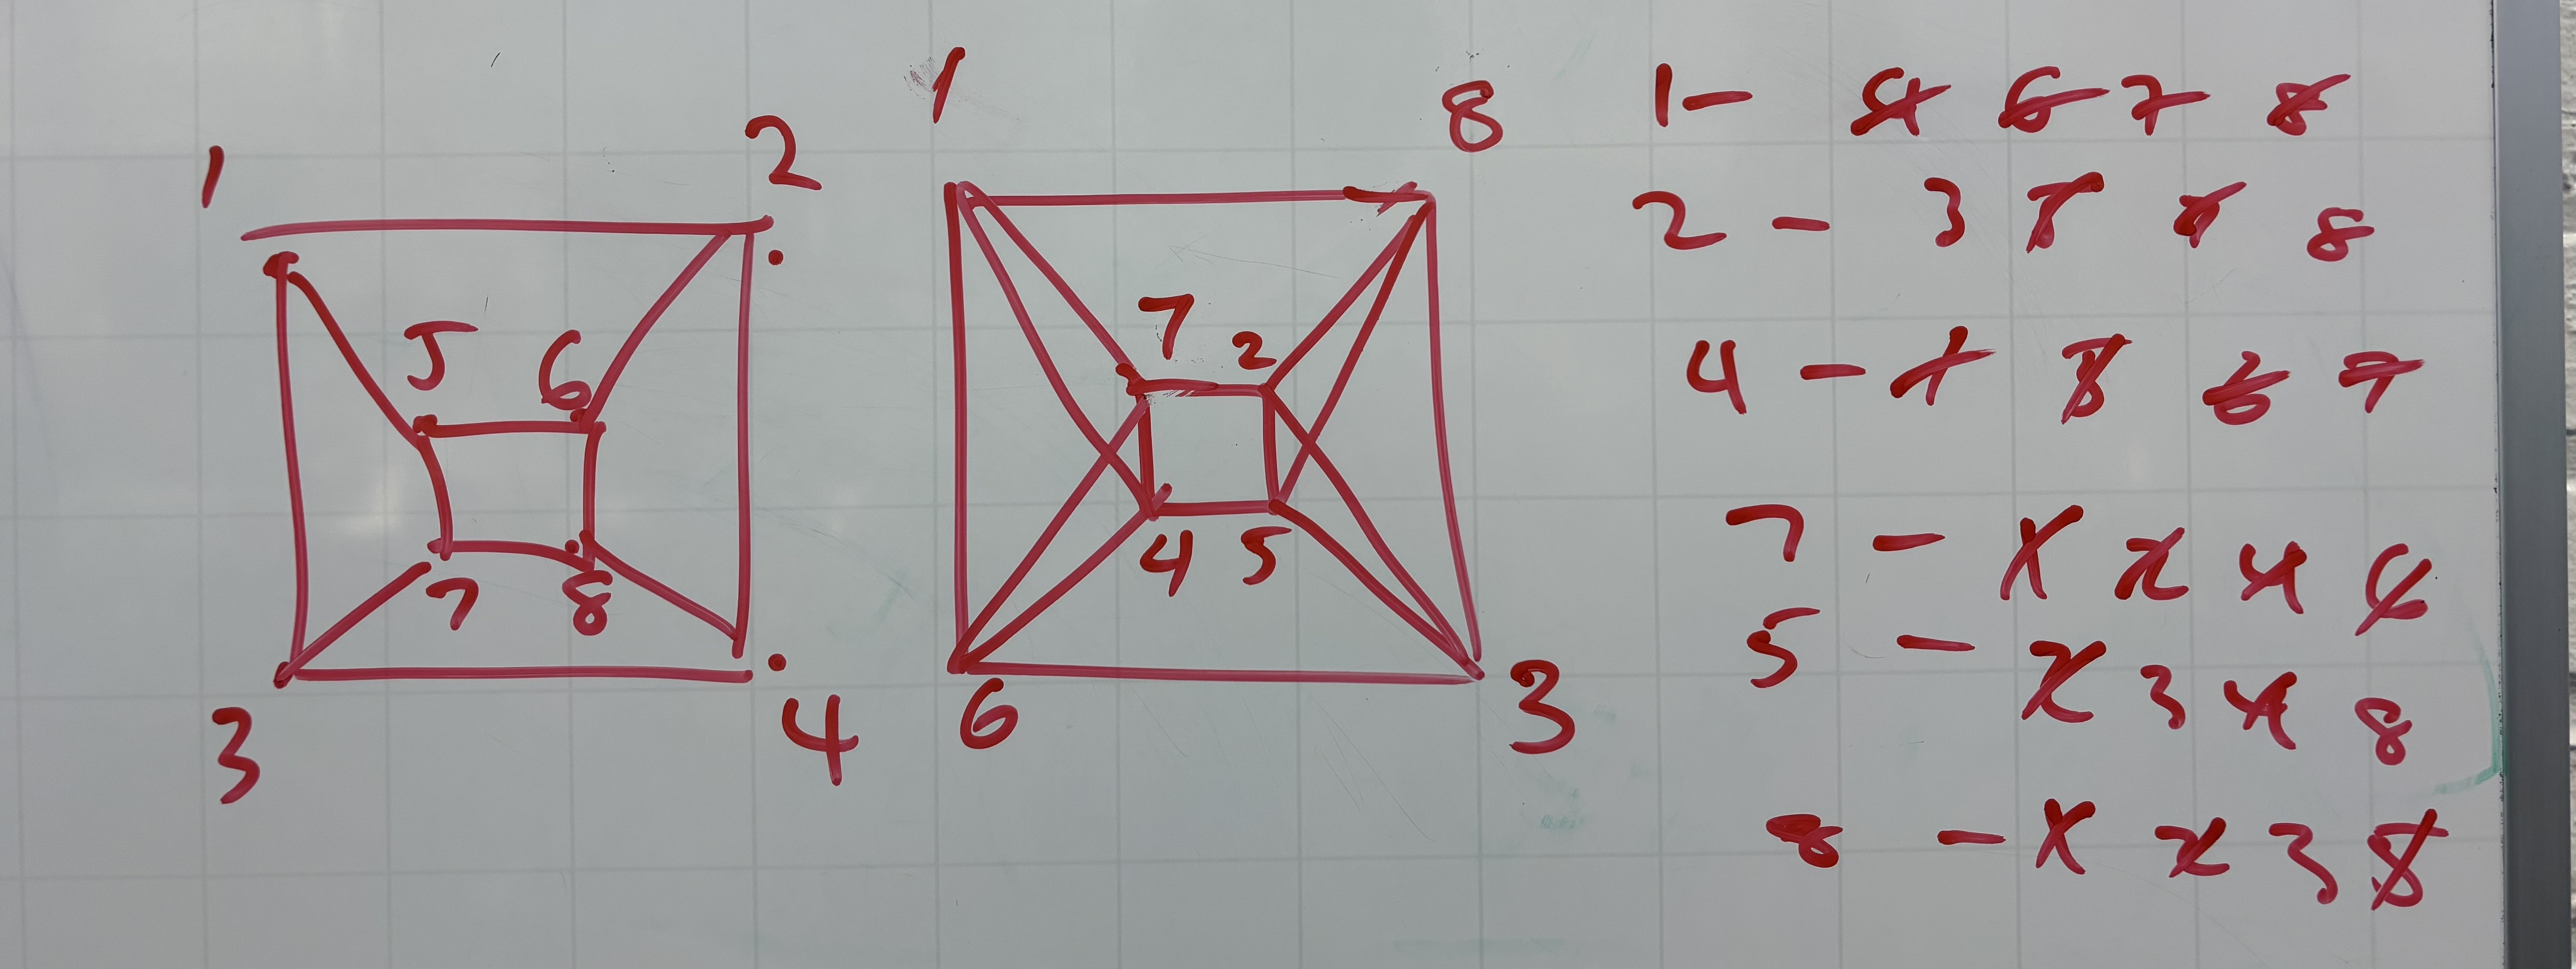
\includegraphics[width=0.8\linewidth]{IMG_3379.jpeg}
		\end{center}

		Notice that any two points are adjacent (and there exists an edge incident to both points) in the left graph if and only if there does not exist an edge incident to both points in the right graph. Thus, the complement of the left graph is isomorphic to the complement of the right graph.

	\item[13.]
		It is not possible for the graph to have any odd cycles. If the coordinates of a vertex have an even number of components equal to $1$, then all vertices it is adjacent to have an odd number of components equal to $1$, and vice versa. In general, the parity of the amount of $1$s in the endpoints of a path are the same if the path is of even length, and different if of odd length. An odd cycle contains an odd number of edges and vertices, so the parity of any point is different from the parity of itself. This is impossible. Since there are no odd cycles, the graph is bipartite. 

	\item[16.]
		Let us consider the complements of the two graphs.
		
		\begin{center}
			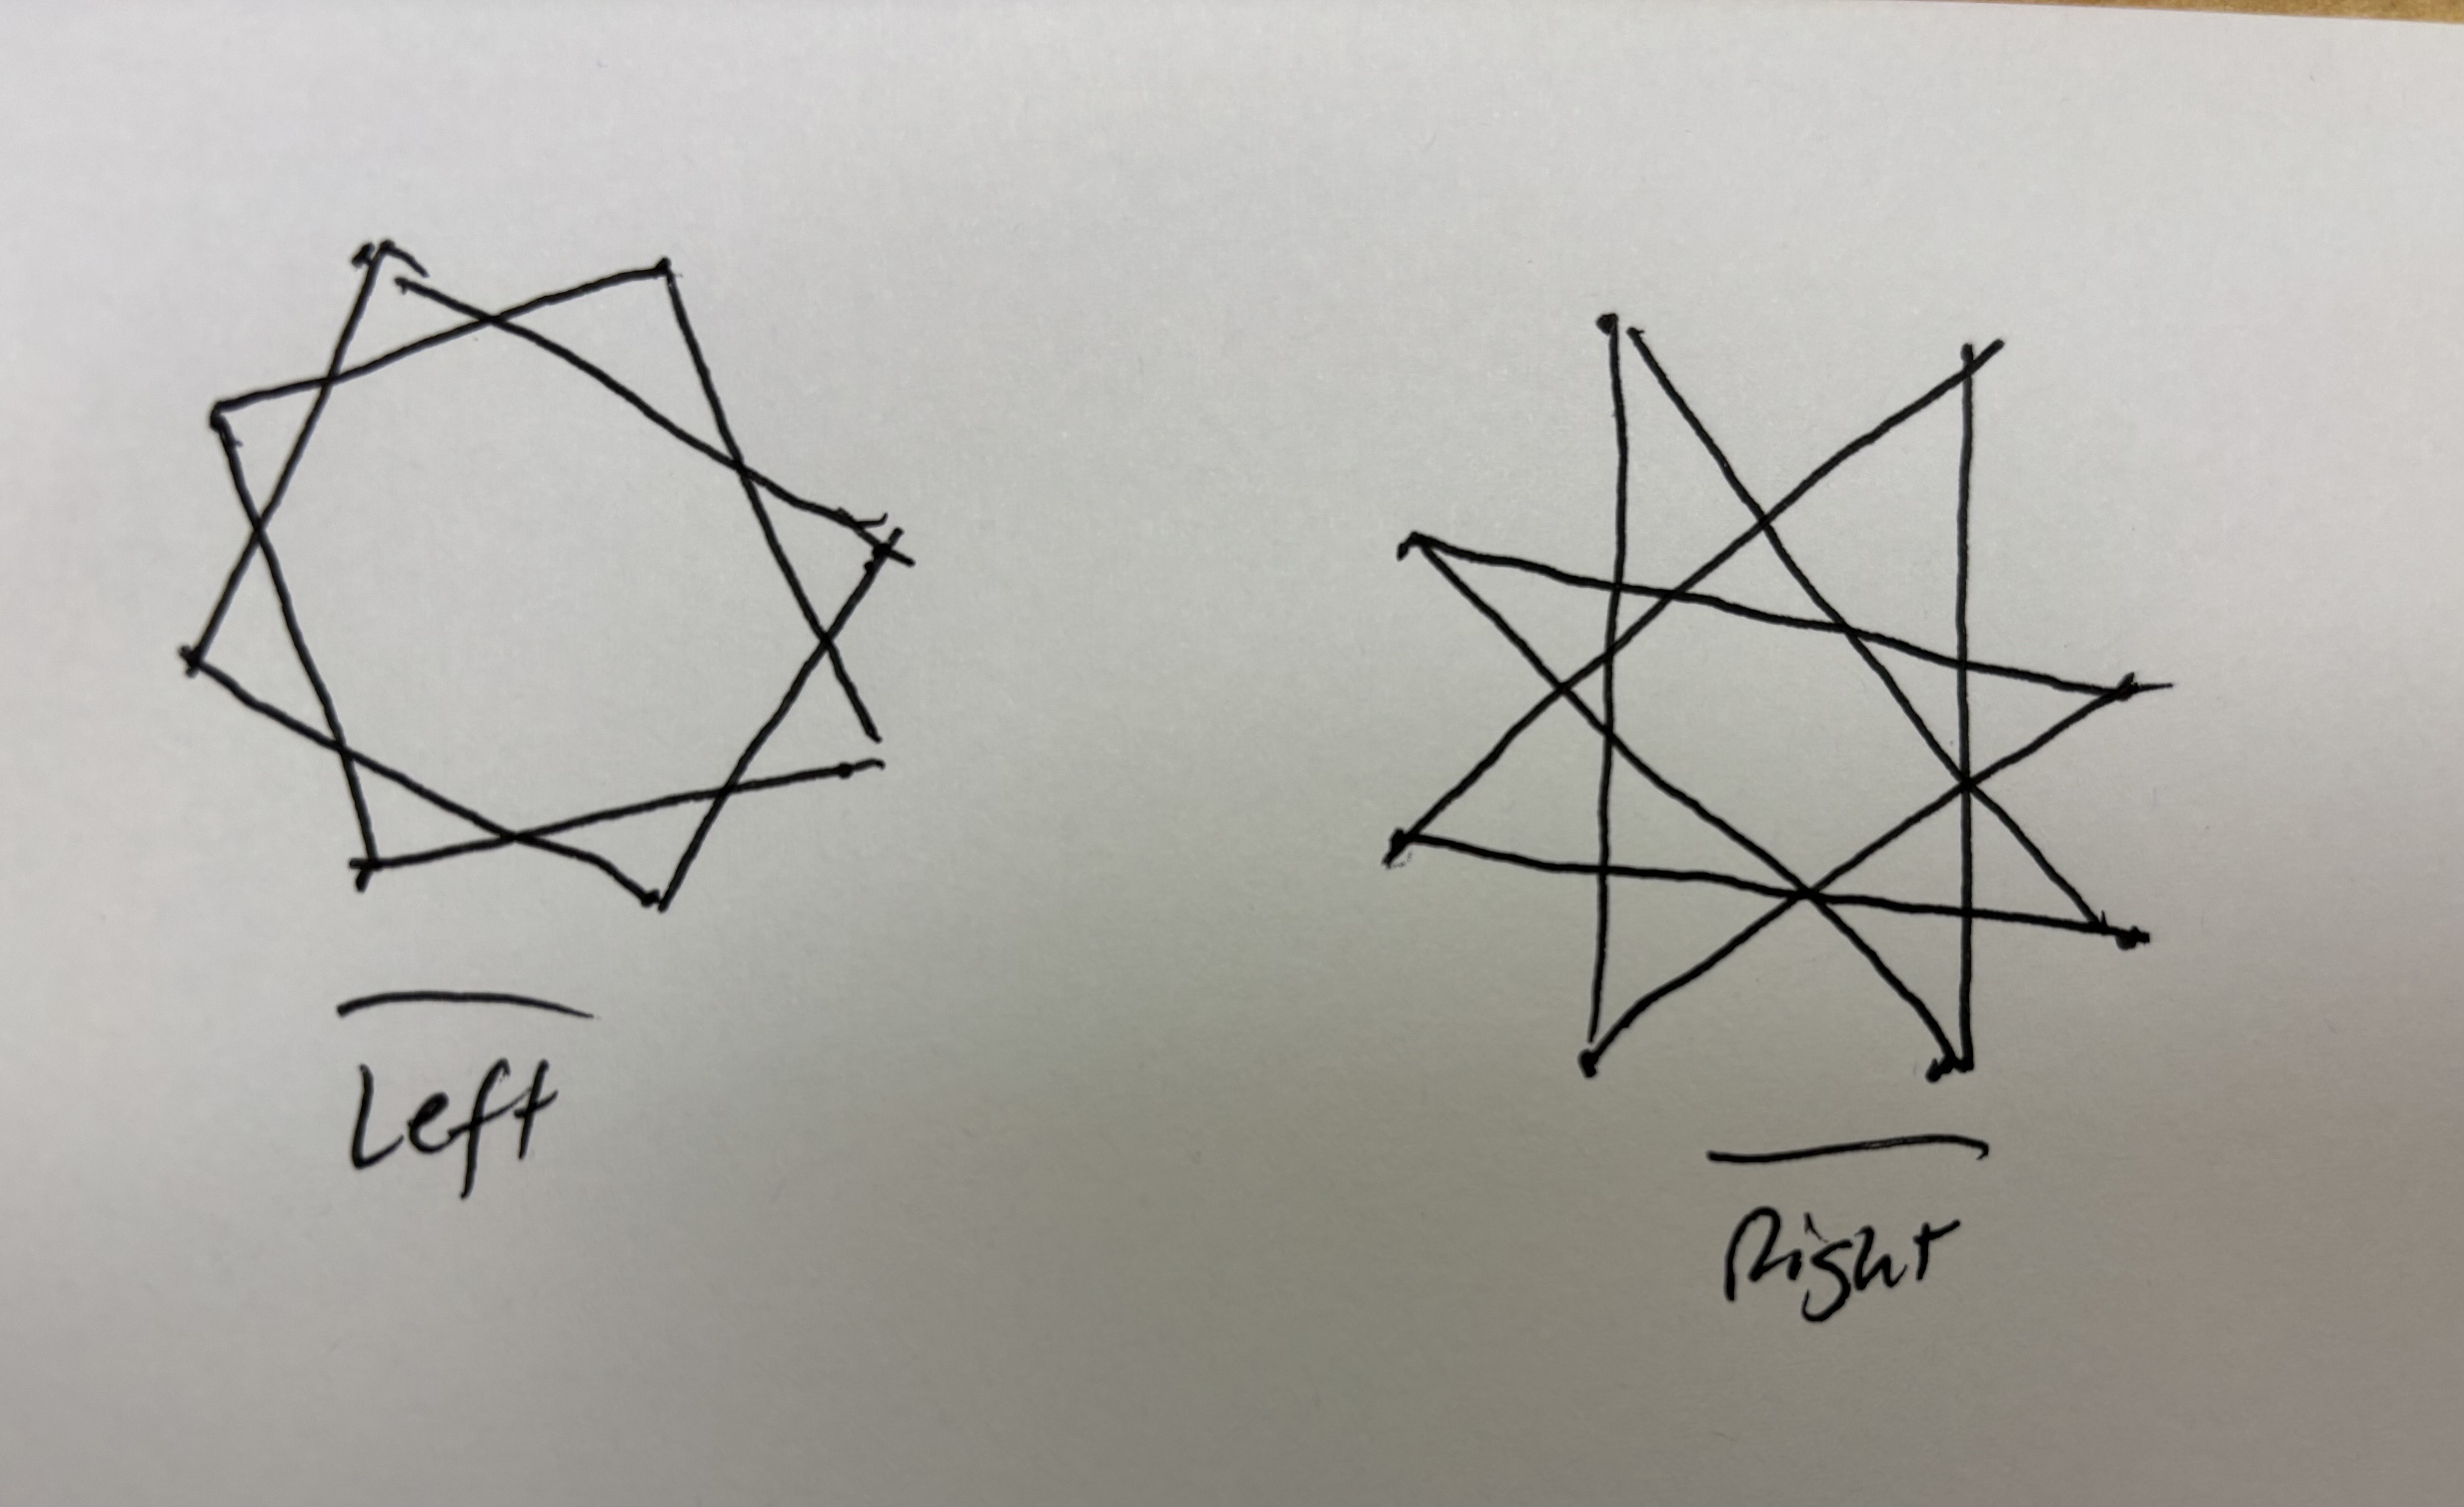
\includegraphics[width=0.8\linewidth]{IMG_3375.jpeg}
		\end{center}

		Notice $\overline{\mathrm{Left}}$ is disconnected $4$, while $\overline{\mathrm{Right}}$ is connected. Since $\overline{\mathrm{Left}}\not\cong \overline{\mathrm{Right}}$, we know that $\mathrm{Left}\not\cong \mathrm{Right}$. The graphs are not isomorphic.

	\item[18.]
		The first two graphs are isomorphic. The graphs are both bipartite and we can use the following bijection: the first partite has $d\to v, e\to u, g\to t, b\to s$ and the second partite has $f\to z, c\to y, a\to x, h\to w$. The first two graphs are not isomorphic to the third graph because the third graph has an odd cycle: $\theta\to\delta\to\gamma\to\beta\to\alpha\to\theta$.


	\item[19.]
		The first graph is not isomorphic to the second and third graphs because the first is bipartite while the second and third graphs are not. The second and third graphs are isomorphic and we can use the following bijection:

		\begin{center}
			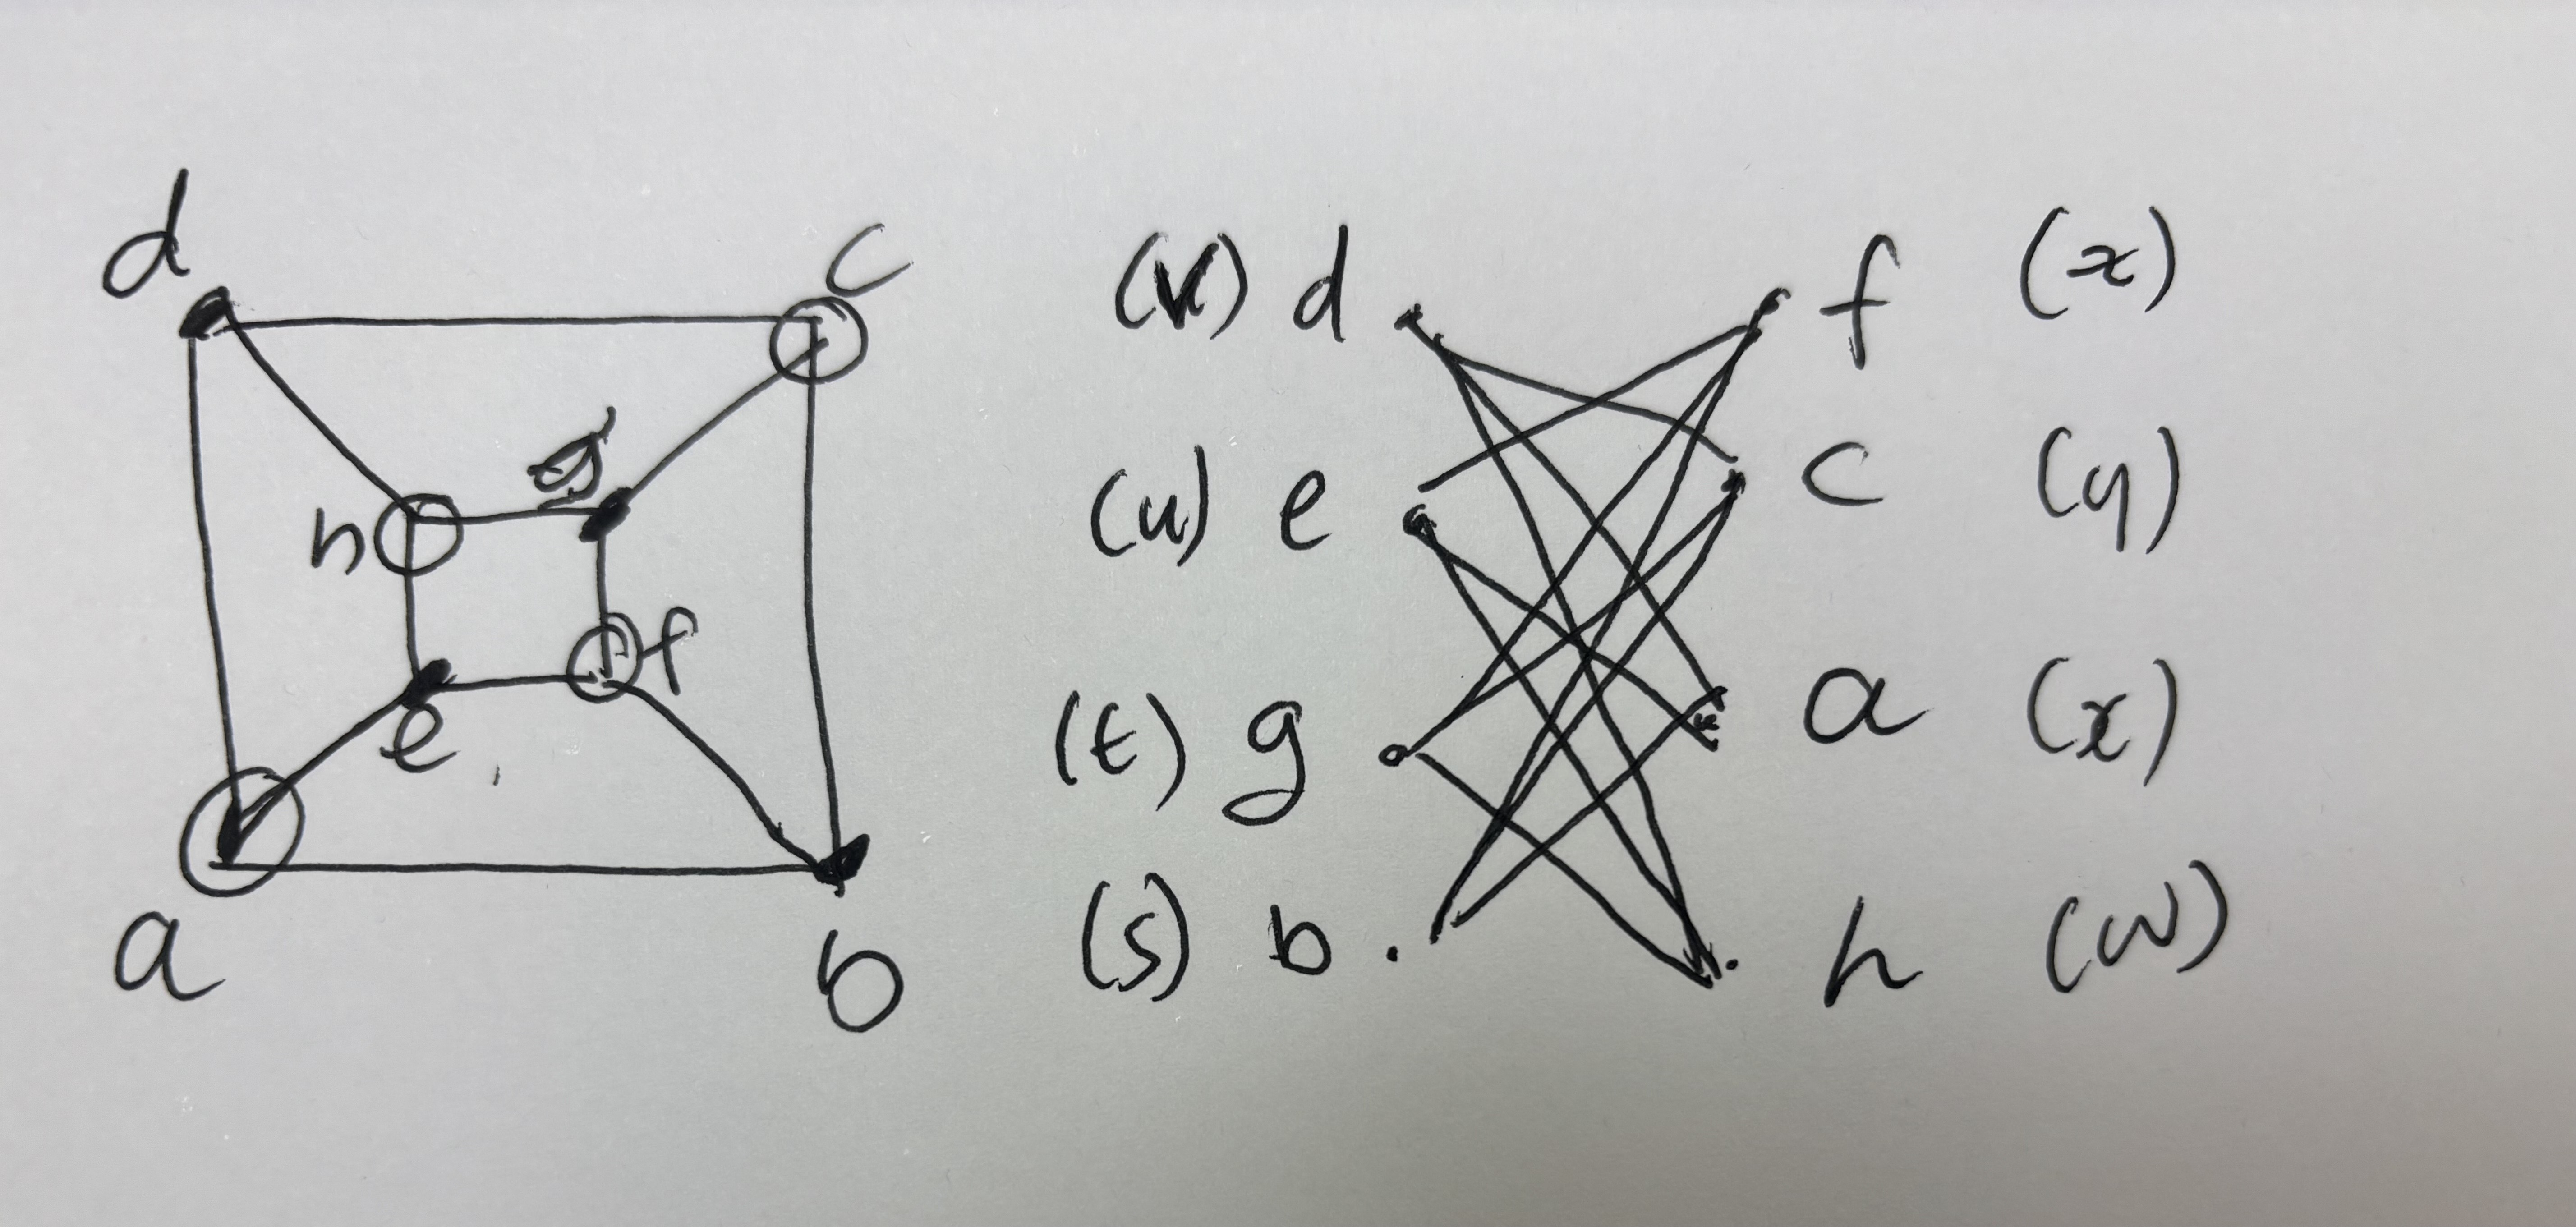
\includegraphics[width=0.8\linewidth]{IMG_3377.jpeg}
		\end{center}


\end{enumerate}

\end{document}
